\subsection{Sharpening Spatial Filters}
Formålet vil oftest være at styrke transitioner i intensitet. Kan anvendes til forskellige ting: 

\begin{itemize}
	\item Electronic printing.
	\item Medical imaging.
	\item Industrial inspection.
	\item Automonous guidance i militær systemer.
\end{itemize}

Til dette bruger vi \textit{spacial differentiation}

\subsubsection{Unsharp Masking og Highboost Filtering}

Bruges af trykpressen. Gør tre ting (også vist på Figur~\ref{fig:unsharp}): 

\begin{enumerate}
	\item Slør originalbilledet.
	\item Træk det slørrede billede fra originalen, resultatet kaldes \textit{masken}.
	\item Tilføj masken til originalen. 
\end{enumerate}

Først skal vi have fundet vores maske. Se Figur~\ref{fig:unsharpeq1}.

\begin{figure}[H]
	\centering
	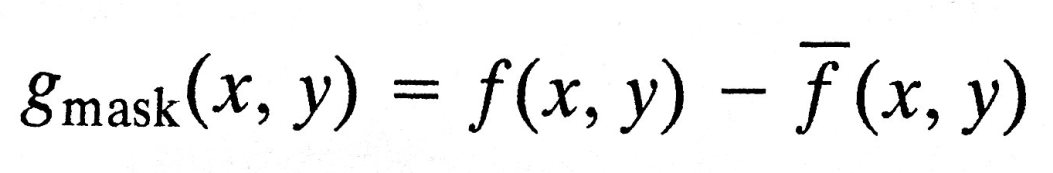
\includegraphics[width=0.4\linewidth]{figs/spm02/unsharpeq1}
	\caption{Her er $\bar{f}(x,y)$ det slørrede billede.}
	\label{fig:unsharpeq1}
\end{figure}

Herefter føjer vi en vægtet udgave af masken til det originale billede, se Figur~\ref{fig:unsharpeq2}.

\begin{figure}[H]
	\centering
	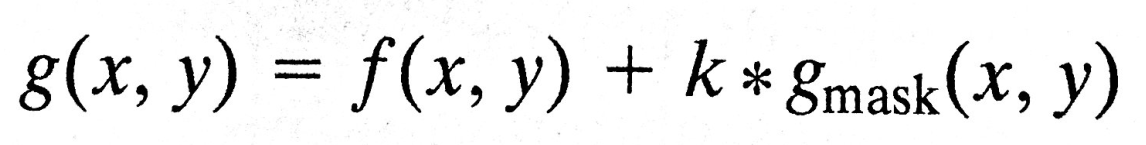
\includegraphics[width=0.4\linewidth]{figs/spm02/unsharpeq2}
	\caption{Det slørrede billedet adderes med en vægt.}
	\label{fig:unsharpeq2}
\end{figure}

I eksemplerne fra Figur~\ref{fig:unsharpeq1}~og~\ref{fig:unsharpeq2} er $k$ vores vægt. Når $k = 1$ er det en \textbf{unsharp masking}. Hvis $k > 1$ kaldes det et \textbf{highboost filter}.

\begin{figure}[H]
	\centering
	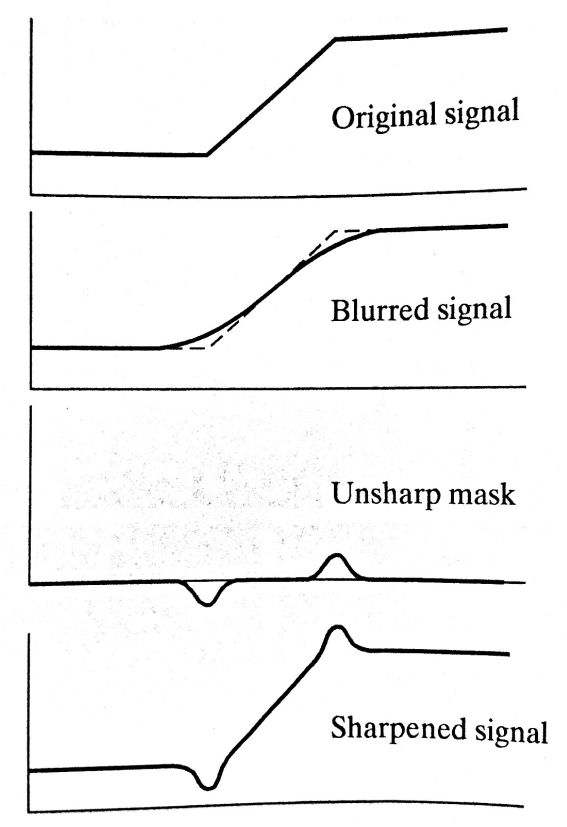
\includegraphics[width=0.4\linewidth]{figs/spm02/unsharp}
	\caption{Hvordan unsharp masking virker.}
	\label{fig:unsharp}
\end{figure}
